% ============================ PART 1: ICE (theory of the 6 Oct talk) ============================
\begin{frame}[plain]
\vfill
\begin{center}
{\Large\bfseries Часть 1. Лёд: метод OA-FM}\\[4mm]
{\color{ink} Теория из доклада 6 октября: почему обычный flow matching плохо использует наблюдения и как это исправить}
\end{center}
\vfill
\end{frame}

\begin{frame}{Постановка задачи}
\begin{columns}[T]
\begin{column}{.5\textwidth}
\small
Восстановить поле концентрации льда $x$ (Баренцево и Карское моря, модель NEMO) на заданный день по
\begin{itemize}
\item фону $x_b$ --- полю той же даты год назад;
\item наблюдениям $y=Hx$ на треках альтиметра SRAL за 3 дня (около 1.3\% площади воды в день).
\end{itemize}
\end{column}
\begin{column}{.46\textwidth}
\small
Оцениваем распределение $p(x\mid y,x_b)$ ансамблем:
\begin{itemize}
\item среднее --- точечная оценка;
\item разброс --- неопределённость;
\item доля членов со льдом --- вероятность льда.
\end{itemize}
\end{column}
\end{columns}
\vspace{1mm}
\centering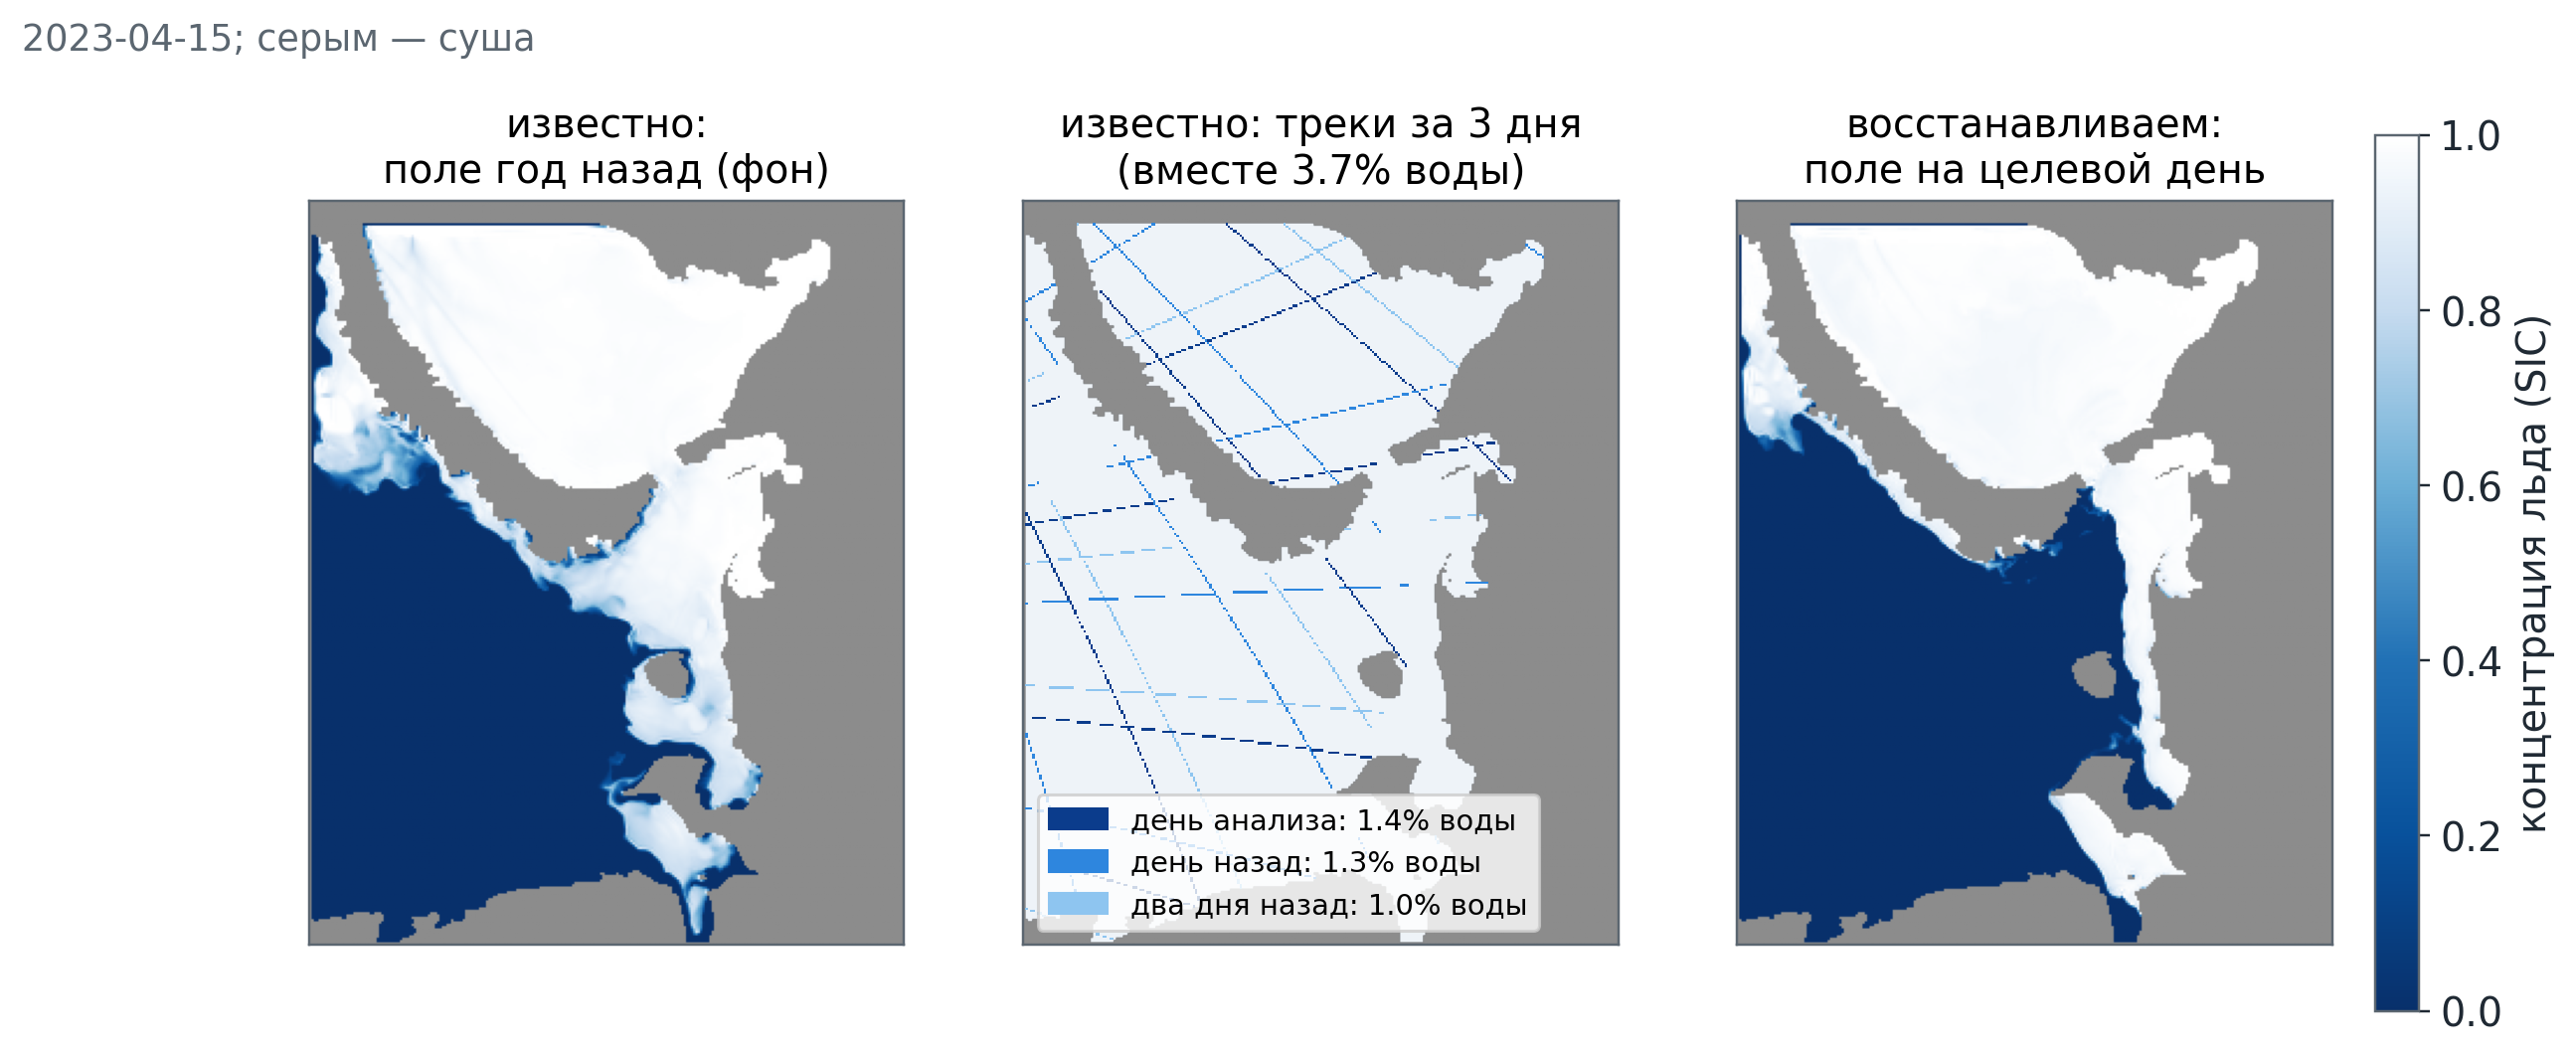
\includegraphics[height=.47\textheight]{figs/ice_setup.png}
\end{frame}

\begin{frame}{Conditional flow matching}
\small
\begin{itemize}
\item Путь от шума к полю: $x_t=(1-t)\,\xi+t\,x$, $\xi\sim\mathcal N(0,I)$, $t\in[0,1]$.
\item Сеть $v_\theta(x_t,t,c)$ обучается на $\E\,\|v_\theta-(x-\xi)\|^2$; оптимум --- $\E[x-\xi\mid x_t,c]$.
\item Условие $c$: фон, значения и маски наблюдений, маска воды, координатная сетка.
\item Генерация: ОДУ $\dot x=v_\theta$ от $t=0$ до $t=1$ (Heun, 32 шага); 16 членов ансамбля из 16 начальных шумов.
\item Сеть --- U-Net; около половины обучающих примеров --- синтетические треки.
\item Данные: обучение 2016--2021, выбор модели 2022, тест 2023.
\end{itemize}
\end{frame}

\begin{frame}{Обычный flow matching плохо использует треки}
\centering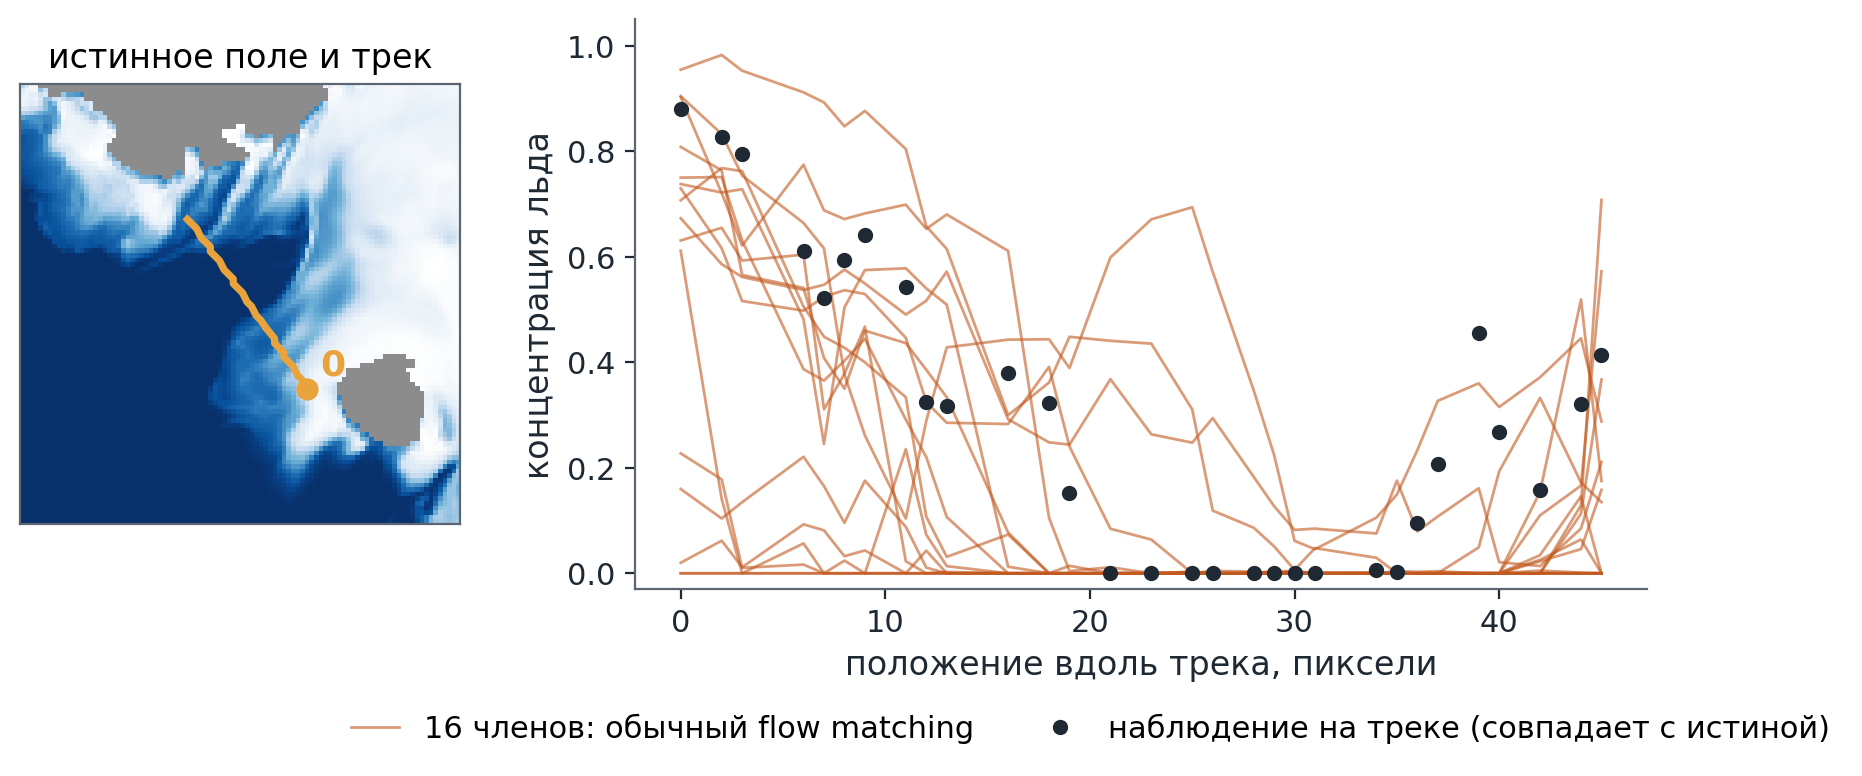
\includegraphics[width=.76\linewidth]{figs/ice_track_problem.png}
\raggedright\small
\begin{itemize}
\item Значение на треке задано точно, но члены ансамбля проходят мимо него: ошибка на треках .12, вдали от треков .23.
\item Треки --- около 4\% пикселей воды, и их вклад в функцию потерь мал.
\item Это не нехватка информации: среднее идеального генератора --- байесовская оценка, и оно не хуже простой копии наблюдения (RMSE .064). У сети --- .124.
\end{itemize}
{\scriptsize\color{ink} 2022 год, точные наблюдения: значение на треке совпадает с истиной. Ошибка --- RMSE одного члена, среднее по 14 дням.\par}
\end{frame}

\begin{frame}{Растянутая шкала концентрации}
\begin{columns}[T]
\begin{column}{.52\textwidth}
\small
Около 55\% пикселей воды --- ровно 0, плотный пак сосредоточен у 1. Непрерывный генератор размазывает ноль в малые положительные значения и выносит пак за 1.

\medskip
Поэтому концентрация генерируется в растянутой шкале
\[z=\tfrac14\,\mathrm{logit}\Big(\frac{\mathrm{SIC}+\varepsilon}{1+2\varepsilon}\Big),\qquad \varepsilon=10^{-3},\]
\[\mathrm{SIC}=\mathrm{clip}\big((1+2\varepsilon)\,\sigma(4z)-\varepsilon,\ 0,\ 1\big).\]
Края шкалы растянуты: значения у 0 и у 1 далеко разнесены. Всё, что сеть выдала ниже образа нуля, переходит ровно в 0.
\end{column}
\begin{column}{.44\textwidth}
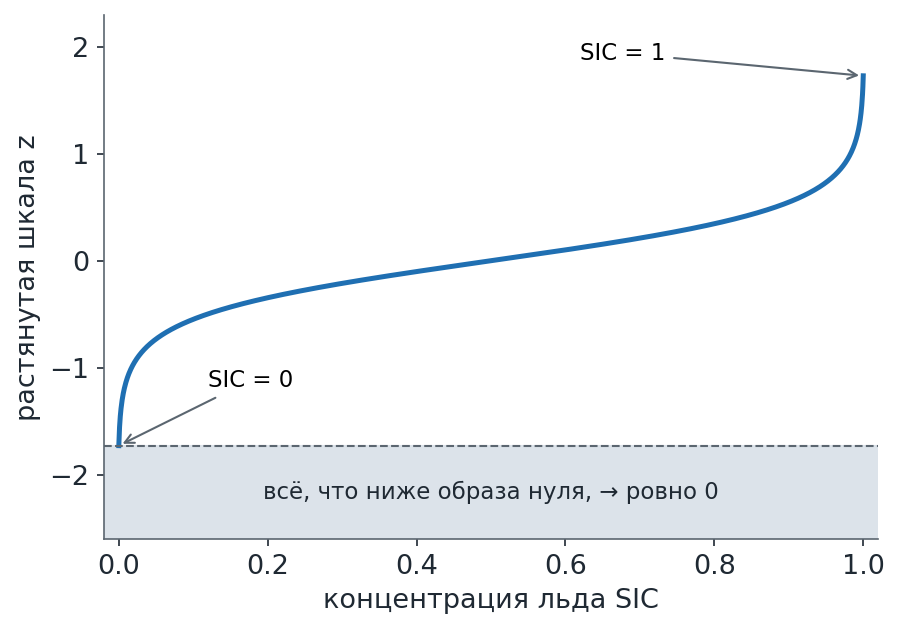
\includegraphics[width=\linewidth]{figs/ice_logit.png}
\end{column}
\end{columns}
\end{frame}

\begin{frame}{Координаты, привязанные к наблюдениям (OA-FM)}
\small
\textbf{Мотивация.} Ширина апостериорного распределения $z$ на треке равна ошибке наблюдения $r\ll1$, вдали от треков --- порядка 1. Поле скоростей должно сжимать ансамбль в $1/r$ раз на 4\% пикселей, и обученная сеть этого не делает.

\textbf{Идея.} Генерировать нормированное отклонение от гауссовой оценки по ближайшему треку:
\[u=\frac{z-m}{s},\qquad m=\rho\,\tilde y,\qquad s=\sqrt{1-\frac{\rho^2}{1+r^2}},\qquad \rho=e^{-d/\ell}.\]
Это оптимальная интерполяция для поля $\mathcal N(0,1)$, коррелированного с треком с коэффициентом $\rho$; $d$ --- расстояние до трека, $\ell=10$ пикселей.
\begin{columns}[T]
\begin{column}{.5\textwidth}
\begin{itemize}
\item В координатах $u$ условная ширина порядка 1 везде: сжимать ансамбль сети не нужно.
\item Ошибка сети $\delta u$ даёт $\delta z=s\,\delta u$; на треке $s\approx r$ --- наблюдение испортить нельзя.
\item Вдали $\rho\to0$ и $u=z$ --- обычная генерация.
\end{itemize}
\end{column}
\begin{column}{.47\textwidth}
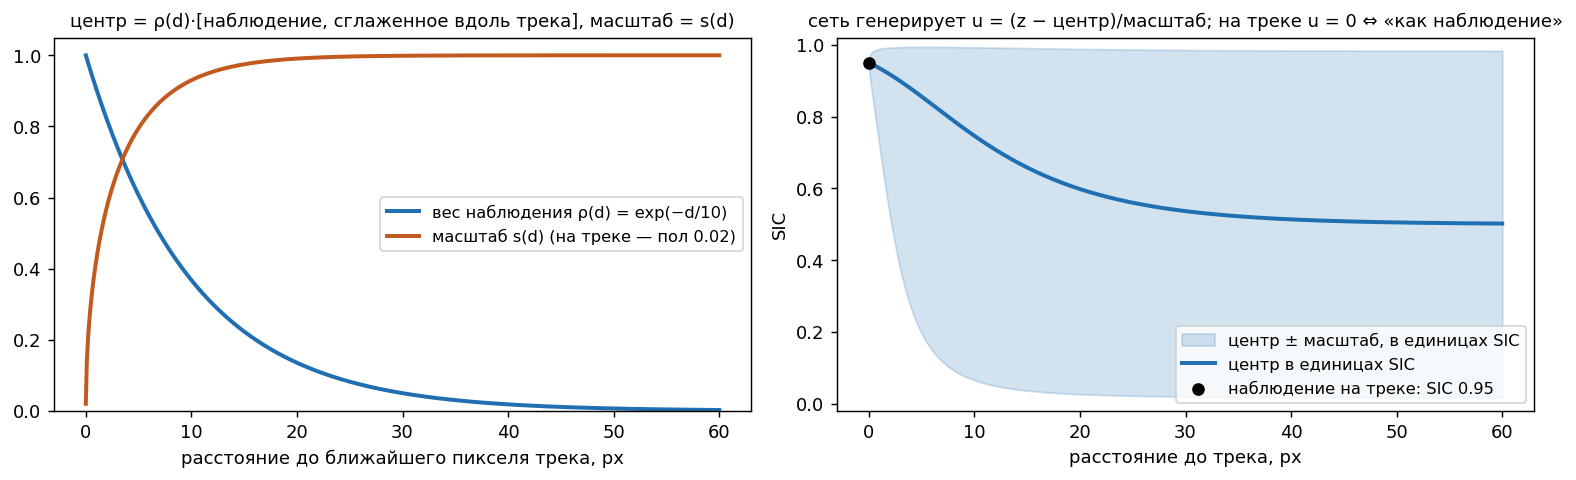
\includegraphics[width=\linewidth]{figs/ice_ap_schematic.png}
\end{column}
\end{columns}
\end{frame}

\begin{frame}{У трека: обычный flow matching и OA-FM}
\centering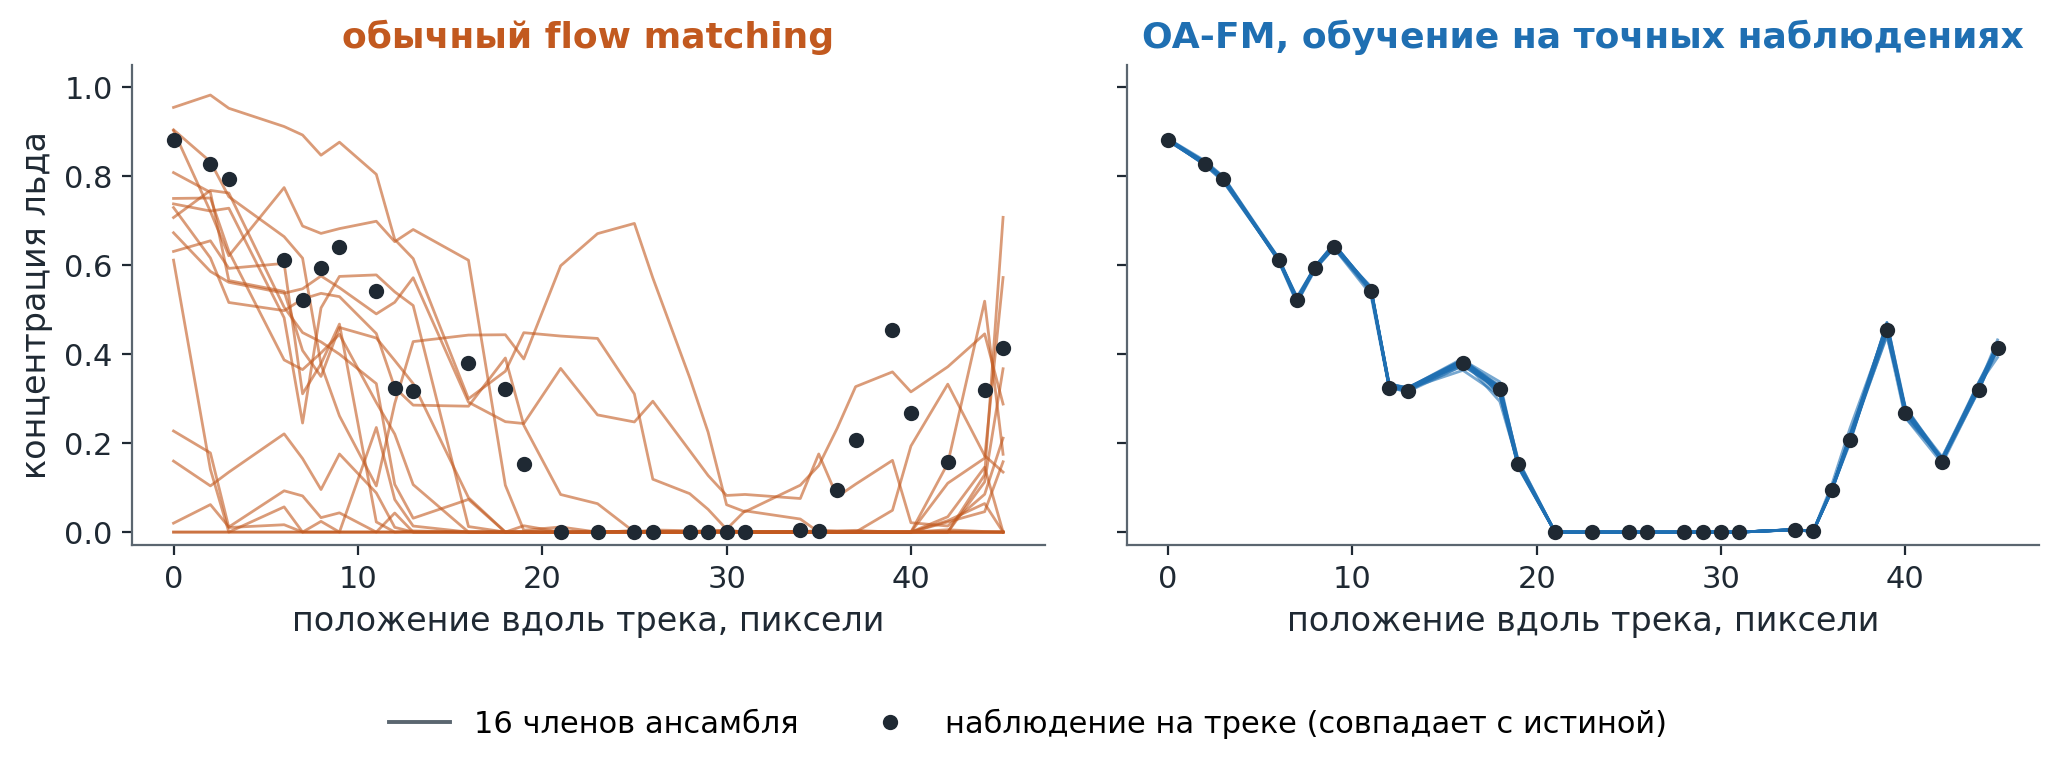
\includegraphics[width=.84\linewidth]{figs/ice_track_fixed.png}
\raggedright\small
\begin{itemize}
\item Тот же трек: все 16 членов OA-FM проходят через наблюдение. Ошибка на треках .12 $\to$ .001, вдали от треков .23 $\to$ .17.
\item Если учить на точных наблюдениях, ансамбль на треках становится слишком уверенным (SSR .03); обучение с моделью ошибки наблюдений даёт SSR .65.
\end{itemize}
\take{Во второй части та же идея --- якорные координаты --- на ERA5. Там видно и то, чего она не решает.}
\end{frame}
